\documentclass[a4paper,12pt]{article}
%----------------------------------------------------------------------------------------
%	DOCUMENT CONFIGURATIONS
%----------------------------------------------------------------------------------------
\usepackage{geometry} % Page margins
\geometry{top=2cm,bottom=2cm,left=2.5cm,right=2.5cm}

\usepackage{xcolor} % Required for specifying colors by name
\definecolor{ocre}{RGB}{243,102,25} %
\definecolor{lightcyan}{rgb}{0.88,1,1}
\definecolor{lightblue}{rgb}{0.8,0.85,1}
\definecolor{gray}{gray}{0.6}
\definecolor{turquoise}{rgb}{0 0.41 0.41}
\definecolor{green}{rgb}{0,0.6,0}
\definecolor{strcol}{rgb}{0.80,0.20,0.20}

% Font Settings
\usepackage{avant} % Use the Avantgarde font for headings
\usepackage{microtype} % Slightly tweak font spacing for aesthetics
%\usepackage[urw-garamond]{mathdesign}
\usepackage{mathpazo}
\usepackage[utf8]{inputenc} % Required for including letters with accents
\usepackage[T1]{fontenc} % Use 8-bit encoding that has 256 glyphs

%\renewcommand{\familydefault}{\sfdefault} %  font sans serif

\usepackage[croatian]{babel} % Croatian language/hyphenation
\usepackage[full]{textcomp} % \textquotesingle


\usepackage{tabularx}

\usepackage{verbatim}%
\usepackage{upquote}%
\usepackage{caption}
\newcommand{\myparagraph}[1]{\paragraph{#1}\mbox{}\\}

\renewcommand{\labelitemii}{$\cdot$} %itemize 2nd level

%----------------------------------------------------------------------------------------
%	VARIOUS RrequQUIRED PACKAGES
%----------------------------------------------------------------------------------------

\usepackage{titlesec} % Allows customization of titles

\usepackage{graphicx} % Required for including pictures
\graphicspath{{./images/}} % Specifies the directory where pictures are stored
\usepackage{float}

\usepackage{tikz} % Required for drawing custom shapes


\usepackage{enumitem} % Customize lists
\setlist{nosep} % Reduce spacing between bullet points and numbered lists

\usepackage{booktabs} % Required for nicer horizontal rules in tables, \toprule, \midrule, and \bottomrule macros 

\usepackage{eso-pic} % Required for specifying an image background in the title page

%\usepackage{wrapfig}
%\usepackage{subfig}

\usepackage[breaklinks]{hyperref}
\usepackage{pdfpages} % za naslovnicu

%\usepackage{xcolor}
\definecolor{dark-red}{rgb}{0.4,0.15,0.15}
\definecolor{dark-blue}{rgb}{0.15,0.15,0.4}
\definecolor{medium-blue}{rgb}{0,0,0.5}
\hypersetup{
    colorlinks=true, pdfborder={0 0 0}, linkcolor={ocre},
    citecolor={ocre}, urlcolor={medium-blue},
    pdftitle = {Operativni sustavi},
    pdfauthor = {Ljiljana Despalatović}
}




%----------------------------------------------------------------------------------------
%	PAGE HEADERS
%----------------------------------------------------------------------------------------

\usepackage{fancyhdr} % Required for header and footer configuration

\pagestyle{fancy}

\fancyhf{} \fancyhead[LE,RO]{\sffamily\normalsize\thepage} % Font setting for the 
\renewcommand{\headrulewidth}{0.5pt} % Width of the rule under the header
\addtolength{\headheight}{2.5pt} % Increase the spacing around the header slightly
\renewcommand{\footrulewidth}{0pt} % Removes the rule in the footer
\fancypagestyle{plain}{\fancyhead{}\renewcommand{\headrulewidth}{0pt}} % Style for when a plain pagestyle is specified

% Removes the header from odd empty pages at the end of chapters
\makeatletter
\renewcommand{\cleardoublepage}{
\clearpage\ifodd\c@page\else
\hbox{}
\vspace*{\fill}
\thispagestyle{empty}
\newpage
\fi}

%----------------------------------------------------------------------------------------
%	THEOREM STYLES
%----------------------------------------------------------------------------------------

 
\usepackage{amsmath,amsfonts,amssymb,amsthm} % For including math equations, theorems, symbols, etc


\newtheoremstyle{ocrenum} % Theorem style name
{20pt} % Space above
{10pt} % Space below
{\normalfont} % Body font
{} % Indent amount
{\small\bf\sffamily\color{ocre}} % Theorem head font
{\;\;} % Punctuation after theorem head
{0.25em} % Space after theorem head
{\small\sffamily\color{ocre}\thmname{#1}\thmnumber{\@ifnotempty{#1}{ }\@upn{#2}} % Theorem text (e.g. Theorem 2.1)
\thmnote{\ {\the\thm@notefont\sffamily\bfseries\color{black}--- #3.}}} % Optional theorem note
\renewcommand{\qedsymbol}{$\blacksquare$} % Optional qed square


% Defines the theorem text style for each type of theorem to one of the three styles above
\theoremstyle{ocrenum}
\newtheorem{problem}{Problem}%[section]
\newtheorem{vjezba}{Vježba}%[section]
\newtheorem{primjer}{Primjer}%[section]
\newtheorem{zadatak}{Zadatak}%[section]
\newtheorem{napomena}{Napomena}%[section]



%--------------------------------------------------
% IMAGES
%--------------------------------------------------
\makeatletter
\g@addto@macro\@floatboxreset\centering
\makeatother

%---------------------------------------------------
% LISTINGS
%---------------------------------------------------
\usepackage{framed}
\usepackage{tikz}
\usepackage{listings}
\lstset{language=C,  keywordstyle=\color{blue!50!black}, columns=flexible, showstringspaces=false, escapechar=@,breaklines=true, lineskip={-1.5pt}, basicstyle=\normalsize\ttfamily, commentstyle=\color{gray},    stringstyle=\color{orange}}
\lstdefinestyle{numbers} {numbers=left, stepnumber=1, numberstyle=\tiny, numbersep=10pt}
\lstdefinestyle{zadatak} {language=C, basicstyle=\normalsize\ttfamily, keywordstyle=\color{blue}, columns=flexible, showstringspaces=false, breaklines=true, lineskip={-1.5pt}}

\usetikzlibrary{decorations}
\usetikzlibrary{calc}
%\pgfmathsetseed{1} % To have predictable results
% Define a background layer, in which the parchment shape is drawn
\pgfdeclarelayer{background}
\pgfsetlayers{background,main}

% define styles for the normal border and the torn border
\tikzset{
  normal border/.style={ocre, rounded corners={0.2cm}, line width={0.05cm}},
  torn border/.style={ocre, rounded corners={0.2cm}, dotted, line width={0.05cm}}}

% Macro to draw the shape behind the text, when it fits completly in the
% page
\def\parchmentframe#1{
\tikz{
  \node[inner sep=0.5em] (A) {#1};  % Draw the text of the node
  %\node[fill=gray!5](box)% Makebox is needed to take the frame added by listings into account
  %\makebox[0.98\textwidth][l]{\box\@tempboxa};
  \begin{pgfonlayer}{background}  % Draw the shape behind
  \draw[normal border] 
        ($(A.south east)-(0.9,0)$) -- ($(A.south west)+(0.6,0)$) -- 
        ($(A.north west)+(0.6,0)$) -- ($(A.north east)-(0.9,0)$) -- cycle;
  \end{pgfonlayer}
  }}

% Macro to draw the shape, when the text will continue in next page
\def\parchmentframetop#1{
\tikz{
  \node[inner sep=2em] (A) {#1};    % Draw the text of the node
  \begin{pgfonlayer}{background}    
  \draw[normal border]              % Draw the ``complete shape'' behind
        %(A.south east) -- 
        ($(A.south west)+(0.6,0)$) -- 
        ($(A.north west)+(0.6,0)$) -- ($(A.north east)-(0.9,0)$) -- ($(A.south east)-(0.9,0)$);
  \draw[torn border]                % Add the torn lower border
         ($(A.south east)-(0.9,0)$) -- ($(A.south west)+(0.6,0)$);
        %($(A.south west)+(0.6,0)$) -- ($(A.south east)+(0.6,0)$) -- cycle;
  \end{pgfonlayer}
  }}

% Macro to draw the shape, when the text continues from previous page
\def\parchmentframebottom#1{
\tikz{
  \node[inner sep=2em] (A) {#1};   % Draw the text of the node
  \begin{pgfonlayer}{background}   
  \draw[normal border]             % Draw the ``complete shape'' behind
        ($(A.north east)-(0.9,0)$) -- ($(A.south east)-(0.9,0)$) -- ($(A.south west)+(0.6,0)$) -- 
        ($(A.north west)+(0.6,0)$);
  \draw[torn border]               % Add the torn upper border
        ($(A.north east)-(0.9,0)$) -- ($(A.north west)+(0.6,0)$);
  \end{pgfonlayer}
  }}

% Macro to draw the shape, when both the text continues from previous page
% and it will continue in next page
\def\parchmentframemiddle#1{
\tikz{
  \node[inner sep=2em] (A) {#1};   % Draw the text of the node
  \begin{pgfonlayer}{background}   
  \draw[normal border]             % Draw the ``complete shape'' behind
        ($(A.south west)+(0.6,0)$) -- ($(A.north west)+(0.6,0)$);
  \draw[normal border]             % Draw the ``complete shape'' behind
        ($(A.north east)-(0.9,0)$) -- ($(A.south east)-(0.9,0)$);        
  \draw[torn border]               % Add the torn lower border
        ($(A.south east)-(0.9,0)$) -- ($(A.south west)+(0.6,0)$);
  \draw[torn border]               % Add the torn upper border
        ($(A.north east)-(0.9,0)$) -- ($(A.north west)+(0.6,0)$);
  \end{pgfonlayer}
  }}

\lstnewenvironment{prototip}[1][]{%
  \lstset{xleftmargin=20pt}
  \def\FrameCommand{\parchmentframe}%
  \def\FirstFrameCommand{\parchmentframetop}%
  \def\LastFrameCommand{\parchmentframebottom}%
  \def\MidFrameCommand{\parchmentframemiddle}%
  %\vskip\baselineskip
  \MakeFramed{\FrameRestore}
  }%
{\endMakeFramed}

\lstnewenvironment{framedcode}[1][]{%
  \lstset{xleftmargin=20pt}
  \def\FrameCommand{\parchmentframe}%
  \def\FirstFrameCommand{\parchmentframetop}%
  \def\LastFrameCommand{\parchmentframebottom}%
  \def\MidFrameCommand{\parchmentframemiddle}%
  %\vskip\baselineskip
  \MakeFramed{\FrameRestore}
  \noindent\tikz\node[inner sep=1ex, draw=ocre,fill=white, rounded corners={0.2cm},  line width={0.05cm}, 
          anchor=west, overlay] at (0em, 2em) {#1};
  }%
{\endMakeFramed}

\lstnewenvironment{framedcodeitem}[1][]{%
  \lstset{xleftmargin=-20pt}
  \def\FrameCommand{\parchmentframe}%
  \def\FirstFrameCommand{\parchmentframetop}%
  \def\LastFrameCommand{\parchmentframebottom}%
  \def\MidFrameCommand{\parchmentframemiddle}%
  %\vskip\baselineskip
  \MakeFramed{\FrameRestore}
  \noindent\tikz\node[inner sep=1ex, draw=ocre,fill=white, rounded corners={0.2cm},  line width={0.05cm}, 
          anchor=west, overlay] at (0em, 2em) {#1};
  }%
{\endMakeFramed}

\lstnewenvironment{framedcodenumber}[1][]{%
  \lstset{style=numbers, xleftmargin=20pt}
  \def\FrameCommand{\parchmentframe}%
  \def\FirstFrameCommand{\parchmentframetop}%
  \def\LastFrameCommand{\parchmentframebottom}%
  \def\MidFrameCommand{\parchmentframemiddle}%
  %\vskip\baselineskip
  \MakeFramed{\FrameRestore}
  \tikz\node[inner sep=1ex, draw=ocre,fill = white, rounded corners={0.2cm}, line width={0.05cm}, 
          anchor=west, overlay] at (0em, 2em) {#1};
  }%
{\endMakeFramed}


\lstnewenvironment{terminall}[1][]{%
  \lstset{style=numbers, xleftmargin=20pt}
  \def\FrameCommand{\parchmentframe}%
  \def\FirstFrameCommand{\parchmentframetop}%
  \def\LastFrameCommand{\parchmentframebottom}%
  \def\MidFrameCommand{\parchmentframemiddle}%
  %\vskip\baselineskip
  \tikzstyle{terminal} = [
    draw=white, text=white, font=courier, fill=black, very thick,
    rectangle, rounded corners, inner sep=2pt, inner ysep=8pt
   ]
   \tikzstyle{terminalTitle} = [
     fill=black, text=white, font=\ttfamily, draw=white
   ]
  \MakeFramed{\FrameRestore}
  \noindent\resizebox{\textwidth}{!}{ % This line fits the box to textwidth
  \tikz\node[inner sep=1ex, draw=ocre,fill = white, rounded corners={0.2cm}, line width={0.05cm}, 
          anchor=west, overlay] at (0em, 2em) {#1};
  }}%
  {\endMakeFramed}

%\usetikzlibrary{shapes}
%\lstset{basicstyle=\ttfamily\footnotesize,breaklines=true}
\newsavebox\terminalbox
\lstnewenvironment{terminal}[1][]
  {\lstset{#1}\setbox\terminalbox=\vbox\bgroup\hsize=0.8\textwidth}
  {\egroup
   \tikzstyle{terminal} = [
    draw=white, text=white, font=courier, fill=black, very thick,
    rectangle, rounded corners, inner sep=2pt, inner ysep=8pt
   ]
   \tikzstyle{terminalTitle} = [
     fill=black, text=white, font=\ttfamily, draw=white
   ]
   \noindent\resizebox{\textwidth}{!}{ % This line fits the box to textwidth
   \begin{tikzpicture}
   \node [terminal] (box){\usebox{\terminalbox}};
   \node[terminalTitle, right=10pt, rounded corners] at (box.north west) {tty: /bin/bash};
   \end{tikzpicture}}
}		


%-----------------------------------------
% TABLES
%-----------------------------------------
\renewcommand{\arraystretch}{0.8} %more/less space between rows




%-----------------------------------------
% VARIOUS
%-----------------------------------------
\usepackage{verbatim}
\usepackage{todonotes}
\usepackage{bitset}


\setlength{\parskip}{6pt} %extra space between paragraphs

% my comments
\newcommand{\ld}[1]{\textcolor[rgb]{1.00,0.50,0.00}
{\noindent\ensuremath{\langle}\textit{napomena: #1}\ensuremath{\rangle}}}

%\author{Ljiljana Despalatovic}
\title{Operativni sustavi}


\linespread{1.3}

\title
{Operativni sustavi\\
Vježba 7}
\date{}

\begin{document}
\maketitle
\todo[inline]{Radna verzija dokumenta (TODO nije zakomentiran) }

\begin{itemize}
\item Na početku vježbe pokrenuti Linux Mint uz pomoć programa \textit{Virtual Machine Launcher}
\item Sve primjere treba izvršiti.
\item Ako nije drugačije navedeno, zadatke treba izvršavati u korisnikovom \texttt{home} direktoriju: \lstinline!~!
\item Na kraju vježbe treba predati povijest naredbi na način kako je opisano u uputama za vježbe.

\end{itemize}
\section{Dozvole i vlasništvo datoteka i direktorija (\textit{file permission})}
\subsection*{Korisnici i grupe}
Da bi se datoteke zaštitile od neovlaštenog pristupa, Linux dozvoljava postavljanje dozvola korištenja datoteka i direktorija. Dozvole se određuju za:
\begin{itemize}
 \item vlasnika datoteke (\textbf{owner})
\item članove grupe kojoj je datoteka dodjeljena (\textbf{group})
\item sve ostale korisnike (\textbf{other}).
\end{itemize}
\begin{primjer} Izvršite \texttt{ls -l}. Prvih 10 znakova označava dozvole korištenja datoteke, zatim je broj koji označava broj linkova, sljedeća polja su vlasnik, grupa, veličina, 
vrijeme zadnje promjene i ime datoteke.

\lstinline!-rwxr-xr-x 1 os os 10103 2010-12-15 10:58 main !

\lstinline!-rw-r--r-- 1 os os   248 2010-12-15 10:58 main.c!
\end{primjer}
U gornjim primjerima:
\begin{itemize}
 \item Prvi znak \texttt{-} ili \texttt{d} označava tip datoteke (datoteka ili direktorij).
\item Sljedeća tri znaka \texttt{rwx} ili \texttt{rw-} označavaju dozvole vlasnika datoteke.
\item Sljedeća tri znaka \texttt{r-x} ili \texttt{r$--$} označavaju dozvole za grupu.
\item Sljedeća tri znaka \texttt{r-x} ili \texttt{r$--$} označavaju dozvole za ostale korisnike.
\end{itemize}
\textbf{Za datoteke:}\\
Troslovna kombinacija slova \texttt{r}, \texttt{w} i \texttt{x} označavaju redom pravo čitanja, pisanja i izvršavanja datoteke.\\
\textbf{Za direktorije:}
 \begin{itemize}
\item 
\texttt{r}: korisnik može vidjeti sadržaj direktorija (npr. sa \texttt{ls} naredbom).                                                                                                            
\item \texttt{w}: korisnik može mijenjati sadržaj direktorija tj. kreirati, brisati i preimenovati datoteke u direktoriju.
\item \texttt{x}: korisnik može koristit direktorij kao svoj tekući direktorij, tj. može ući u njega naredbom \texttt{cd}. 
\end{itemize}
\subsection*{Mijenjanje dozvola}
Sintaksa \texttt{chmod <MODE> <ime\_datoteke>}
\\
\texttt{<MODE>} može biti napisan simbolički npr. \texttt{chmod go-rx kopija.c} ili oktalno npr. \texttt{chmod 700 kopija.c}.\\
\subsubsection*{Simbolički}\texttt{chmod <TKO OPERATOR STO> <ime\_datoteke>}\\
\texttt{<TKO>} može biti:
\begin{itemize}
 \item \textbf{u} user
\item \textbf{g} grupa
\item \textbf{o} ostali
\item \textbf{a} svi
\end{itemize}
\texttt{<OPERATOR>} može biti:
\begin{itemize}
 \item \textbf{+} dodavanje prava
\item \textbf{-} oduzimanje prava
\item \textbf{=} skidanje svih prava i dodavanje specificiranih
\end{itemize}
\texttt{<STO>} može biti \textbf{r}, \texttt{w} i \textbf{x}.

\begin{primjer}{Primjer simboličkog načina pridjeljivanja prava korištenja:}
\begin{itemize}
 \item \texttt{chmod u=rw,go=r kopija.c} - user dobija pravo pisanja i čitanja, a grupa i ostali samo čitanja.
\item \texttt{chmod a+x main} - svi dobiju pravo izvršavanja uz već postojeća prava.
\end{itemize}
\end{primjer}
\subsubsection*{Oktalno zapisivanje prava korištenja}
\texttt{chmod <ZZZ> <ime\_datoteke>}\\
Z - oktalna znamenka (znamenka između 0 i 7)
%\begin{figure}
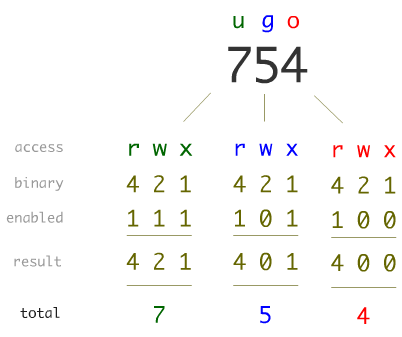
\includegraphics[scale=0.3]{07_File_perm_03.png}
%\end{figure}

\begin{primjer}Primjer oktalnog načina pridjeljivanja prava korištenja:
\begin{itemize}
 \item \texttt{chmod 644 kopija.c} - user dobija pravo pisanja i čitanja, a grupa i ostali samo čitanja.
\item \texttt{chmod 755 main} - svi dobiju pravo izvršavanja uz već postojeća prava.
\end{itemize}
\end{primjer}
\begin{zadatak} Nakon svake izvršene naredbe u primjerima i zadacima, izvršite naredbu \texttt{ls -l} kako bi vidjeli promjene.
\begin{itemize}
\item U direktoriju \texttt{vjezba7} kreirajte datoteku main.c u kojoj će biti neki c program.
\item Iskompajlirajte ga: \texttt{gcc -o main main.c} 
\item Napravite kopiju datoteke \texttt{main.c}. Neka se kopija zove \texttt{kopija.c}.
\end{itemize}
\end{zadatak}
\begin{zadatak}
Datoteci \texttt{kopija.c} dodijelite takva prava da samo \texttt{user} može mijenjati datoteku. 
\end{zadatak}
\begin{zadatak}
Datoteci \texttt{main} dodijelite takva prava da samo \texttt{user} i pripadajuća grupa mogu izvršavati datoteku tj. program \texttt{main}. 
\end{zadatak}
\begin{zadatak}
Datoteci \texttt{main} skinite pravo mijenjanja za \texttt{usera}. Pokušajte pokrenuti program \texttt{./main}. 
\end{zadatak}
\begin{zadatak}
Kreirajte direktorij \texttt{test} i u njega kopirajte datoteku \texttt{main}. Direktoriju \texttt{test} skinite pravo pisanja \texttt{w}. 
Kopirajte datoteku \texttt{main.c} u njega. Kakav je rezultat i zašto? 
\end{zadatak}

\begin{comment}

\vfill
\begin{itemize}
\renewcommand{\labelitemi}{\textbf{$\rightarrow$}}
\item Popis svih pokrenutih naredbi eksportirajte u datoteku imena \texttt{prezime\_ime\_vj7.txt}. Uploadajte datoteku na \href{https://moodle.oss.unist.hr/course/view.php?id=133}{http://moodle.oss.unist.hr}.
\end{itemize}

\end{comment}

\end{document}